\subsection{Complete-Method Results and Generalization}
\begin{table*}[!t]\centering\scriptsize\setlength{\tabcolsep}{3pt}\renewcommand{\arraystretch}{1.18}
\caption{S6 accuracy (\%) under matching restoration: G-L for PAMF-Sup, G-LU for external Full+PL and PAMF-REPL. Complete recipes and G permissions differ; values are not single-component causal effects. Mean $\pm$ sample SD over three F seeds.}
\label{tab:repl-main}\begin{tabular*}{\textwidth}{@{\extracolsep{\fill}}lrrrrrr@{}}\toprule
Partition / shift & RIEI & DRIFT-v2 & IB-RFF & SDG & PAMF-Sup & PAMF-REPL\\\midrule
F0 / Date & \pmv{57.87}{1.40} & \pmv{70.54}{0.52} & \pmv{90.50}{0.16} & \pmv{91.45}{0.21} & \pmv{90.99}{0.23} & \pmv{92.31}{0.22}\\
F0 / RX & \pmv{56.73}{0.91} & \pmv{60.75}{4.42} & \pmv{62.21}{2.86} & \pmv{67.12}{0.97} & \pmv{77.36}{0.55} & \pmv{78.29}{0.97}\\
F0 / Both & \pmv{57.11}{0.72} & \pmv{59.78}{3.53} & \pmv{62.84}{0.98} & \pmv{65.66}{0.76} & \pmv{75.34}{0.71} & \pmv{76.73}{0.88}\\
F1 / Date & \pmv{72.81}{0.59} & \pmv{75.44}{3.21} & \pmv{81.23}{2.87} & \pmv{77.95}{1.57} & \pmv{83.36}{0.36} & \pmv{84.27}{1.08}\\
F1 / RX & \pmv{57.39}{1.31} & \pmv{53.60}{3.33} & \pmv{55.68}{1.82} & \pmv{58.84}{1.15} & \pmv{65.84}{0.12} & \pmv{66.83}{0.66}\\
F1 / Both & \pmv{58.24}{1.72} & \pmv{55.47}{4.73} & \pmv{57.30}{2.11} & \pmv{58.67}{1.43} & \pmv{65.20}{0.34} & \pmv{66.91}{1.50}\\
F2 / Date & \pmv{65.28}{1.62} & \pmv{69.95}{2.40} & \pmv{87.61}{0.52} & \pmv{89.75}{0.30} & \pmv{87.46}{0.37} & \pmv{88.74}{0.21}\\
F2 / RX & \pmv{62.96}{1.55} & \pmv{57.15}{4.16} & \pmv{65.00}{2.36} & \pmv{64.34}{1.25} & \pmv{74.99}{0.25} & \pmv{74.64}{0.05}\\
F2 / Both & \pmv{61.53}{2.55} & \pmv{54.67}{4.23} & \pmv{64.16}{1.63} & \pmv{64.10}{1.91} & \pmv{75.25}{0.87} & \pmv{73.99}{0.86}\\
ManyRx / Date & \pmv{31.89}{6.04} & \pmv{46.16}{4.69} & \pmv{72.07}{0.42} & \pmv{75.00}{0.74} & \pmv{77.49}{0.31} & \pmv{77.16}{0.21}\\
ManyRx / RX & \pmv{28.70}{5.43} & \pmv{43.34}{3.64} & \pmv{64.99}{0.77} & \pmv{66.07}{0.75} & \pmv{71.96}{0.03} & \pmv{72.25}{0.39}\\
ManyRx / Both & \pmv{29.39}{7.82} & \pmv{40.92}{3.94} & \pmv{62.31}{0.31} & \pmv{66.48}{0.36} & \pmv{69.26}{0.77} & \pmv{70.15}{0.84}\\\bottomrule\end{tabular*}\end{table*}
Table~\ref{tab:repl-main} reports the main physical partitions. On F0 cross-RX, PAMF-REPL plus DURA reaches \pmv{78.29}{0.97}\% S6 accuracy, compared with \pmv{67.12}{0.97}\% for the fixed SDG D recipe. The within-seed difference is \pmv{11.16}{1.08} percentage points (pp), positive for all three F seeds. The corresponding REPL raw clean and raw S6 values are \pmv{86.56}{0.65}\% and \pmv{70.77}{0.45}\%; after restoration clean is \pmv{86.62}{0.69}\%. We retain every scene rather than infer robustness from clean alone.


\begin{figure}[!t]
\centering
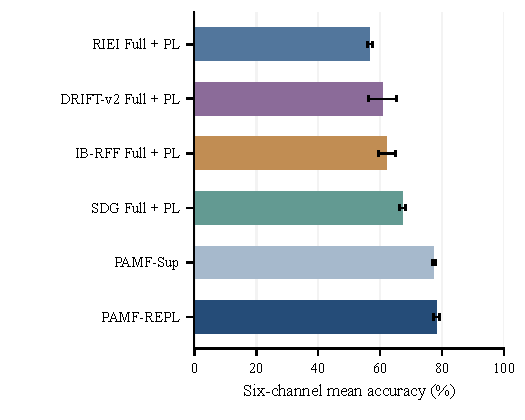
\includegraphics[width=\columnwidth]{images/repl/Fig04_F0_cross_rx_restored.pdf}
\caption{Fixed complete recipes on F0 cross-RX. Error bars are three-F-seed sample SD. The external D cell is fixed in advance, not chosen by target rank.}
\label{fig:repl-main}
\end{figure}
The matched Sup/G-L system reaches \pmv{77.36}{0.55}\%, making the complete-system difference \pmv{0.93}{0.97} pp. This comparison changes both F and G permissions. Holding G-LU fixed, REPL minus Sup is \pmv{-0.09}{1.28} pp and REPL minus ordinary PL is \pmv{-0.23}{0.95} pp. Their S6 means are nonpositive on 6/11 and 8/11 contracts, respectively. Thus the data support strong restored complete-system performance relative to these fixed external recipes, but not uniformly beneficial semi-supervision or an optimal D cell for every method.


\begin{figure}[!t]
\centering
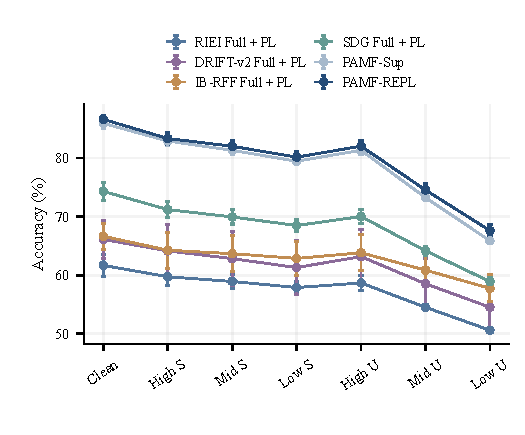
\includegraphics[width=\columnwidth]{images/repl/Fig11_F0_seven_views_restored.pdf}
\caption{All seven F0 cross-RX observations. Clean also passes through the restorer. Suburban (S) and urban (U) impairments are simulations; scene-specific weaknesses and clean changes remain visible.}
\label{fig:repl-scenes}
\end{figure}
REPL cross-RX S6 is \pmv{66.83}{0.66}\% on F1 and \pmv{74.64}{0.05}\% on F2. ManyRx cross-RX S6 Macro-F1 is \pmv{72.27}{0.42}\%, using all ten classes. The label-fraction and natural source-count curves retain their negative and nonmonotonic differences. The source-count axis changes source data volume as well as RX diversity, so it does not isolate receiver count at a fixed labeling budget.


\begin{figure}[!t]
\centering
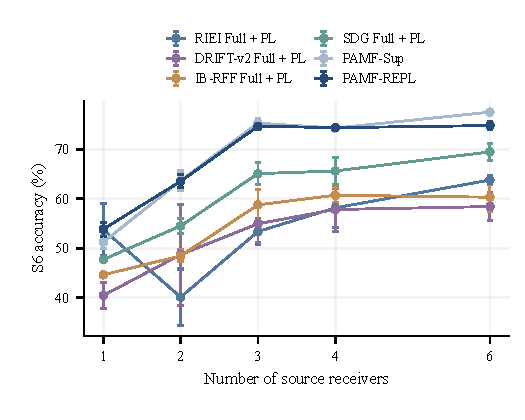
\includegraphics[width=\columnwidth]{images/repl/Fig07_source_cross_rx_restored.pdf}
\caption{Natural-budget source-count study with six fixed target RX. Only measured m=1,2,3,4,6 points are shown; F0 is not inserted as a five-source point.}
\label{fig:repl-source}
\end{figure}
\subsection{Functional Groups and REPL Mechanisms}
The core groups are defined by function: A is labeled-source cross-RX CRIC, B is labeled-source paired symmetric KL, and C is the complete REPL U objective, including its U consistency and contrastive terms. Main rows 111/011/101/110 are accompanied by all eight combinations for marginal effects and interactions. C0 does not construct a U loader. The matched 000 CE skeleton keeps 768 L packet forwards/update.

\begin{table}[!t]\centering\scriptsize\setlength{\tabcolsep}{3pt}\caption{Core removal results on F0 cross-RX (\%). G-LU still consumes U when F has C0.}\label{tab:repl-core}\begin{tabular*}{\columnwidth}{@{\extracolsep{\fill}}lrrr@{}}\toprule Row & Raw clean & Raw S6 & G-LU S6\\\midrule
111: Full & \pmv{86.56}{0.65} & \pmv{70.77}{0.45} & \pmv{78.29}{0.97}\\
011: no A & \pmv{86.62}{0.99} & \pmv{70.58}{0.16} & \pmv{78.62}{1.08}\\
101: no B & \pmv{86.22}{0.66} & \pmv{70.35}{1.20} & \pmv{78.02}{0.49}\\
110: no C & \pmv{85.94}{0.84} & \pmv{71.29}{0.90} & \pmv{78.37}{0.43}\\\bottomrule\end{tabular*}\end{table}
For raw clean, full-minus-removal differences are \pmv{-0.05}{0.83}, \pmv{0.34}{1.17} and \pmv{0.63}{1.49} pp for A/B/C, respectively. The marginal B/C effects across the full factorial are \pmv{1.14}{0.72} and \pmv{1.60}{1.09} pp, while BC is \pmv{-1.69}{0.49} pp. Marginal and full-conditional effects answer different questions; these interactions preclude an additive interpretation. SD with three seeds is not a significance test.


\begin{figure}[!t]
\centering
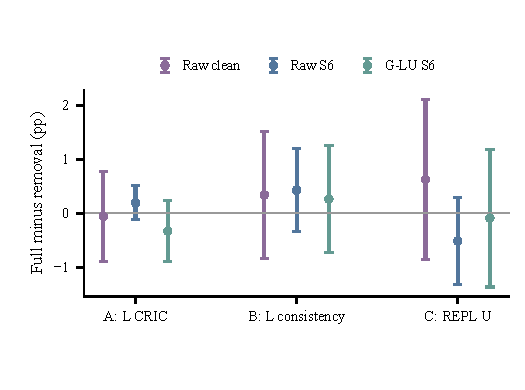
\includegraphics[width=\columnwidth]{images/repl/Fig12_core_conditional_effects.pdf}
\caption{Full 111 minus 011/101/110. Raw and restored effects are separate; negative and seed-dependent contributions are retained.}
\label{fig:repl-core}
\end{figure}
The internal C ablations remove U style, gradient protection, joint-feature contrast or receiver extrapolation, each with the same E50 trajectory and head. The no-extrapolation row reuses the exact matching prior Joint160 model rather than retraining it. These are the four mechanisms of the selected REPL method; obsolete EMA/neighbor/strong-gate controls are not relabeled as REPL ablations. Full-minus-removal effects and all three seeds are supplied for every population/view/route.


\begin{figure}[!t]
\centering
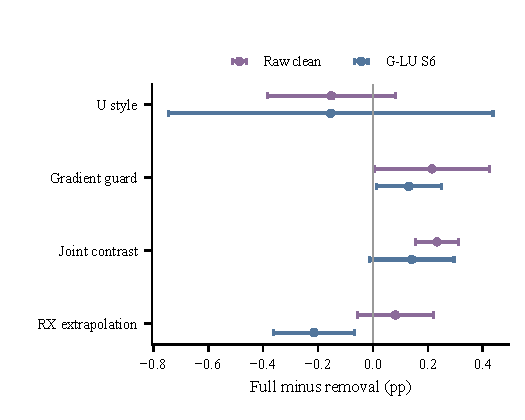
\includegraphics[width=\columnwidth]{images/repl/Fig14_REPL_inner_mechanisms.pdf}
\caption{Actual REPL component removals on F0 cross-RX. The same within-seed full/removal pairing is used before computing three-seed SD.}
\label{fig:repl-inner}
\end{figure}
Seven labeled-branch controls examine shallow-only, intermediate-only and joint-only CRIC, single stochastic forwarding, no As, As KL enabled and no raw CE. They remain diagnostic appendix rows. Single forwarding changes computation/stochastic exposure; no-raw-CE changes CE dose; the strict CE recipe changes the complete supervised objective. We do not attribute these complete-recipe differences to one isolated factor.

\subsection{Physical Structure and Restorer Controls}
The nine architectures comprise full, single time route, no time, shuffled time, no signature, no PA, no reference, fixed wrong reference and COV-X3. Each is evaluated under both full REPL and strict supervised CE, three seeds per layer. All physically matched readers use raw/G-L/G-LU; primary matching is G-LU for REPL and G-L for strict CE. The two layers differ in supervised dose and losses and are not interchangeable controls.


\begin{figure}[!t]
\centering
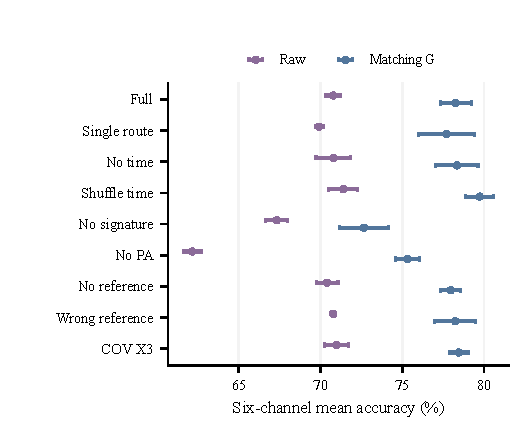
\includegraphics[width=\columnwidth]{images/repl/Fig15_REPL_structure.pdf}
\caption{Architecture sensitivity under the complete REPL recipe. Matching restoration is G-LU; all raw and alternative-G-role results remain in the tables.}
\label{fig:repl-structure}
\end{figure}
We reconnect seven already trained G controls to REPL for all three populations, without retraining G. Their paired F/G seeds differ from the fixed-G default summary, so the variation is not a pure-G estimate or a complete replicated copy-by-KD factorial. The three-source $3F\times3G$ grid gives diagonal S6 \pmv{74.54}{1.15}\% on cross-RX; all nine cells are supplied, and same-F raw stratified CMs agree across the extra G readouts. Only the three diagonal pairs are three complete-system training repetitions.

Source-only diagnostics evaluate the identical 720 L packets from 90 TX/RX/day strata under 11 interventions for 111 F0 models. They read no U/target and fit no diagnostic head. Default-head flips and feature/reference distances quantify sensitivity; they do not prove complete hardware disentanglement, and simulated PA distortion is not assumed to preserve TX identity.

\subsection{Efficiency and Accounting}
\begin{table}[!t]\centering\footnotesize\caption{Exclusive RTX3090 B1 timings (ms), pooled across five rounds. F is eager; GF uses the existing optimized graph engine. These are different execution paths, not an isolated speedup caused by G.}\label{tab:repl-latency}\begin{tabular*}{\columnwidth}{@{\extracolsep{\fill}}lrrr@{}}\toprule Case & Median & P95 & CPU round trip\\\midrule
Sup F & 7.4029 & 7.7351 & 7.6140\\
Sup GF & 4.5629 & 4.5821 & 4.6176\\
PL F & 7.4310 & 7.7949 & 7.3536\\
PL GF & 4.5657 & 4.5854 & 4.6222\\
REPL F & 7.3070 & 7.7823 & 7.2362\\
REPL GF & 4.5246 & 4.5639 & 4.6032\\\bottomrule\end{tabular*}\end{table}
The updated optimized G+REPL path has B1 wall median 4.524556ms, P95 4.563896ms and CPU round-trip median 4.603213ms. Four exclusive panels cover 1175 case-rounds: REPL/strict-CE nine-architecture readers, matching Sup/ordinary-PL controls and seven existing G combinations. Batch sizes are 1/8/32/64/128; five rounds repeat timing, not training seeds. We retain 329000 timed calls and 395975 total inference invocations including warm-up, cold and transfer checks. Training-only REPL mechanisms add no inference-specific parameters. Loaded-module parameter counts and co-resident memory are retained with their measurement scope; they are not claims of active deployment MACs or isolated-model VRAM.


\begin{figure}[!t]
\centering
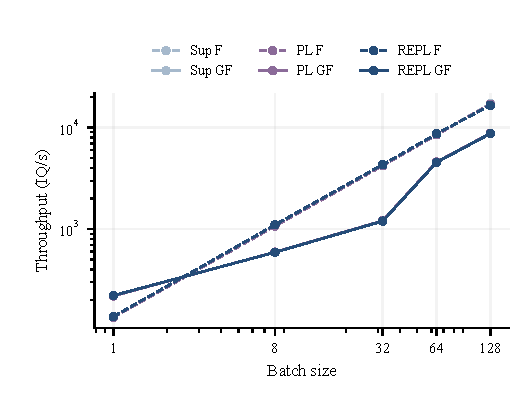
\includegraphics[width=\columnwidth]{images/repl/Fig19_measured_throughput.pdf}
\caption{Measured exclusive-device throughput. The eager-F and optimized-GF paths are explicitly separated; shared-cache classifier timing is not substituted for online G+F timing.}
\label{fig:repl-throughput}
\end{figure}
The 189 new F completions use 84 unique shared E20 prefixes and 8670 unique new model-epochs (1924740 updates), totaling 265.956426 shared-worker elapsed hours. The 201 logical F rows include 12 frozen F0 models and reused prefixes; summing logical cumulative costs would double-count shared stages. Each source stage, actual U acceptance and L-forward dose is retained. All C0/strict rows have zero U exposure. DURA adds zero new training and zero new restored-IQ caches in this rerun; its original training ancestry and shared-cache production are historical costs, not free computation. Known matched G costs are listed separately; the original fixed F0 G-LU ancestor timing is incompletely serialized and remains missing rather than inferred as zero.

\subsection{Evidence Boundaries}
All negative gains, zero external PL acceptance and nonmonotonic source/label curves remain available. The benchmark shares WiSig acquisition hardware; synthetic residual channels do not establish in-orbit validity. Post-selection F0 clean performance, conditional F-seed variation, distinct G permissions and exposure differences constrain causal claims. The supplementary package contains the full frozen CMs/net corrections, source/epoch counters, timing samples and a pure-standard-library replay; IQ, model weights, per-sample target truth and private controller state are excluded.
\appendices
\section{Complete PAMF Diagnostic Rows}
\par\medskip\noindent\begin{minipage}{\columnwidth}\centering\scriptsize\setlength{\tabcolsep}{2pt}\makeatletter\def\@captype{table}\makeatother\caption{Labeled-branch diagnostic recipes: F0 cross-RX accuracy (\%). Complete rows retain every seed; exposure differences are described in the main text.}\begin{tabular*}{\columnwidth}{@{\extracolsep{\fill}}lrrr@{}}\toprule Recipe & Raw clean & Raw S6 & G S6\\\midrule
Full & \pmv{86.56}{0.65} & \pmv{70.77}{0.45} & \pmv{78.29}{0.97}\\
As KL on & \pmv{86.56}{1.25} & \pmv{71.00}{0.18} & \pmv{78.66}{1.11}\\
joint only & \pmv{86.50}{1.24} & \pmv{70.29}{0.22} & \pmv{78.39}{1.46}\\
middle only & \pmv{86.46}{1.42} & \pmv{70.81}{0.14} & \pmv{78.43}{1.17}\\
shallow only & \pmv{86.42}{1.09} & \pmv{71.00}{0.59} & \pmv{78.54}{0.99}\\
single forward & \pmv{86.62}{0.98} & \pmv{71.18}{0.50} & \pmv{78.31}{0.62}\\
without As & \pmv{86.26}{0.39} & \pmv{42.93}{5.96} & \pmv{78.29}{0.84}\\
without raw CE & \pmv{86.89}{1.44} & \pmv{71.19}{0.52} & \pmv{78.54}{1.12}\\\bottomrule\end{tabular*}\end{minipage}\par\medskip
\par\medskip\noindent\begin{minipage}{\columnwidth}\centering\scriptsize\setlength{\tabcolsep}{2pt}\makeatletter\def\@captype{table}\makeatother\caption{REPL architecture layer: F0 cross-RX accuracy (\%). Complete rows retain every seed; exposure differences are described in the main text.}\begin{tabular*}{\columnwidth}{@{\extracolsep{\fill}}lrrr@{}}\toprule Recipe & Raw clean & Raw S6 & G S6\\\midrule
Full & \pmv{86.56}{0.65} & \pmv{70.77}{0.45} & \pmv{78.29}{0.97}\\
COV X3 & \pmv{86.70}{0.66} & \pmv{70.97}{0.73} & \pmv{78.46}{0.57}\\
NO PA & \pmv{82.48}{0.13} & \pmv{62.16}{0.54} & \pmv{75.32}{0.74}\\
NO REFERENCE & \pmv{85.07}{0.91} & \pmv{70.40}{0.67} & \pmv{77.97}{0.62}\\
NO SIGNATURE & \pmv{82.06}{0.78} & \pmv{67.32}{0.67} & \pmv{72.65}{1.51}\\
NO TIME & \pmv{86.12}{1.77} & \pmv{70.79}{1.06} & \pmv{78.34}{1.29}\\
SHUFFLE TIME & \pmv{88.08}{0.85} & \pmv{71.39}{0.87} & \pmv{79.74}{0.86}\\
SIG TIME & \pmv{85.57}{1.41} & \pmv{69.91}{0.24} & \pmv{77.70}{1.72}\\
WRONG REFERENCE & \pmv{86.10}{0.72} & \pmv{70.78}{0.16} & \pmv{78.24}{1.26}\\\bottomrule\end{tabular*}\end{minipage}\par\medskip
\par\medskip\noindent\begin{minipage}{\columnwidth}\centering\scriptsize\setlength{\tabcolsep}{2pt}\makeatletter\def\@captype{table}\makeatother\caption{Strict-CE architecture layer: F0 cross-RX accuracy (\%). Complete rows retain every seed; exposure differences are described in the main text.}\begin{tabular*}{\columnwidth}{@{\extracolsep{\fill}}lrrr@{}}\toprule Recipe & Raw clean & Raw S6 & G S6\\\midrule
full & \pmv{83.69}{1.04} & \pmv{71.40}{0.40} & \pmv{75.69}{0.53}\\
COV X3 & \pmv{83.49}{0.98} & \pmv{71.68}{0.80} & \pmv{75.65}{0.47}\\
NO PA & \pmv{78.74}{0.45} & \pmv{64.19}{0.71} & \pmv{72.08}{0.59}\\
NO REFERENCE & \pmv{82.49}{0.88} & \pmv{70.82}{0.41} & \pmv{74.95}{0.78}\\
NO SIGNATURE & \pmv{83.36}{1.36} & \pmv{70.52}{0.51} & \pmv{75.54}{0.87}\\
NO TIME & \pmv{83.60}{1.31} & \pmv{70.84}{0.56} & \pmv{75.26}{0.37}\\
SHUFFLE TIME & \pmv{84.89}{1.51} & \pmv{72.16}{0.86} & \pmv{77.38}{0.69}\\
SIG TIME & \pmv{84.14}{0.35} & \pmv{70.55}{0.58} & \pmv{75.47}{1.20}\\
WRONG REFERENCE & \pmv{83.06}{0.63} & \pmv{71.06}{0.44} & \pmv{75.17}{0.61}\\\bottomrule\end{tabular*}\end{minipage}\par\medskip
The supplementary 27 standalone figures additionally show the complete core, internal removals, source geometry, fairness four-cell contrasts, measured architecture timing and all external Full A/B/C/D cells. They retain the same physical partitions and metric definitions as the main text.
